% Created by tikzDevice version 0.12.6 on 2025-02-05 15:21:59
% !TEX encoding = UTF-8 Unicode
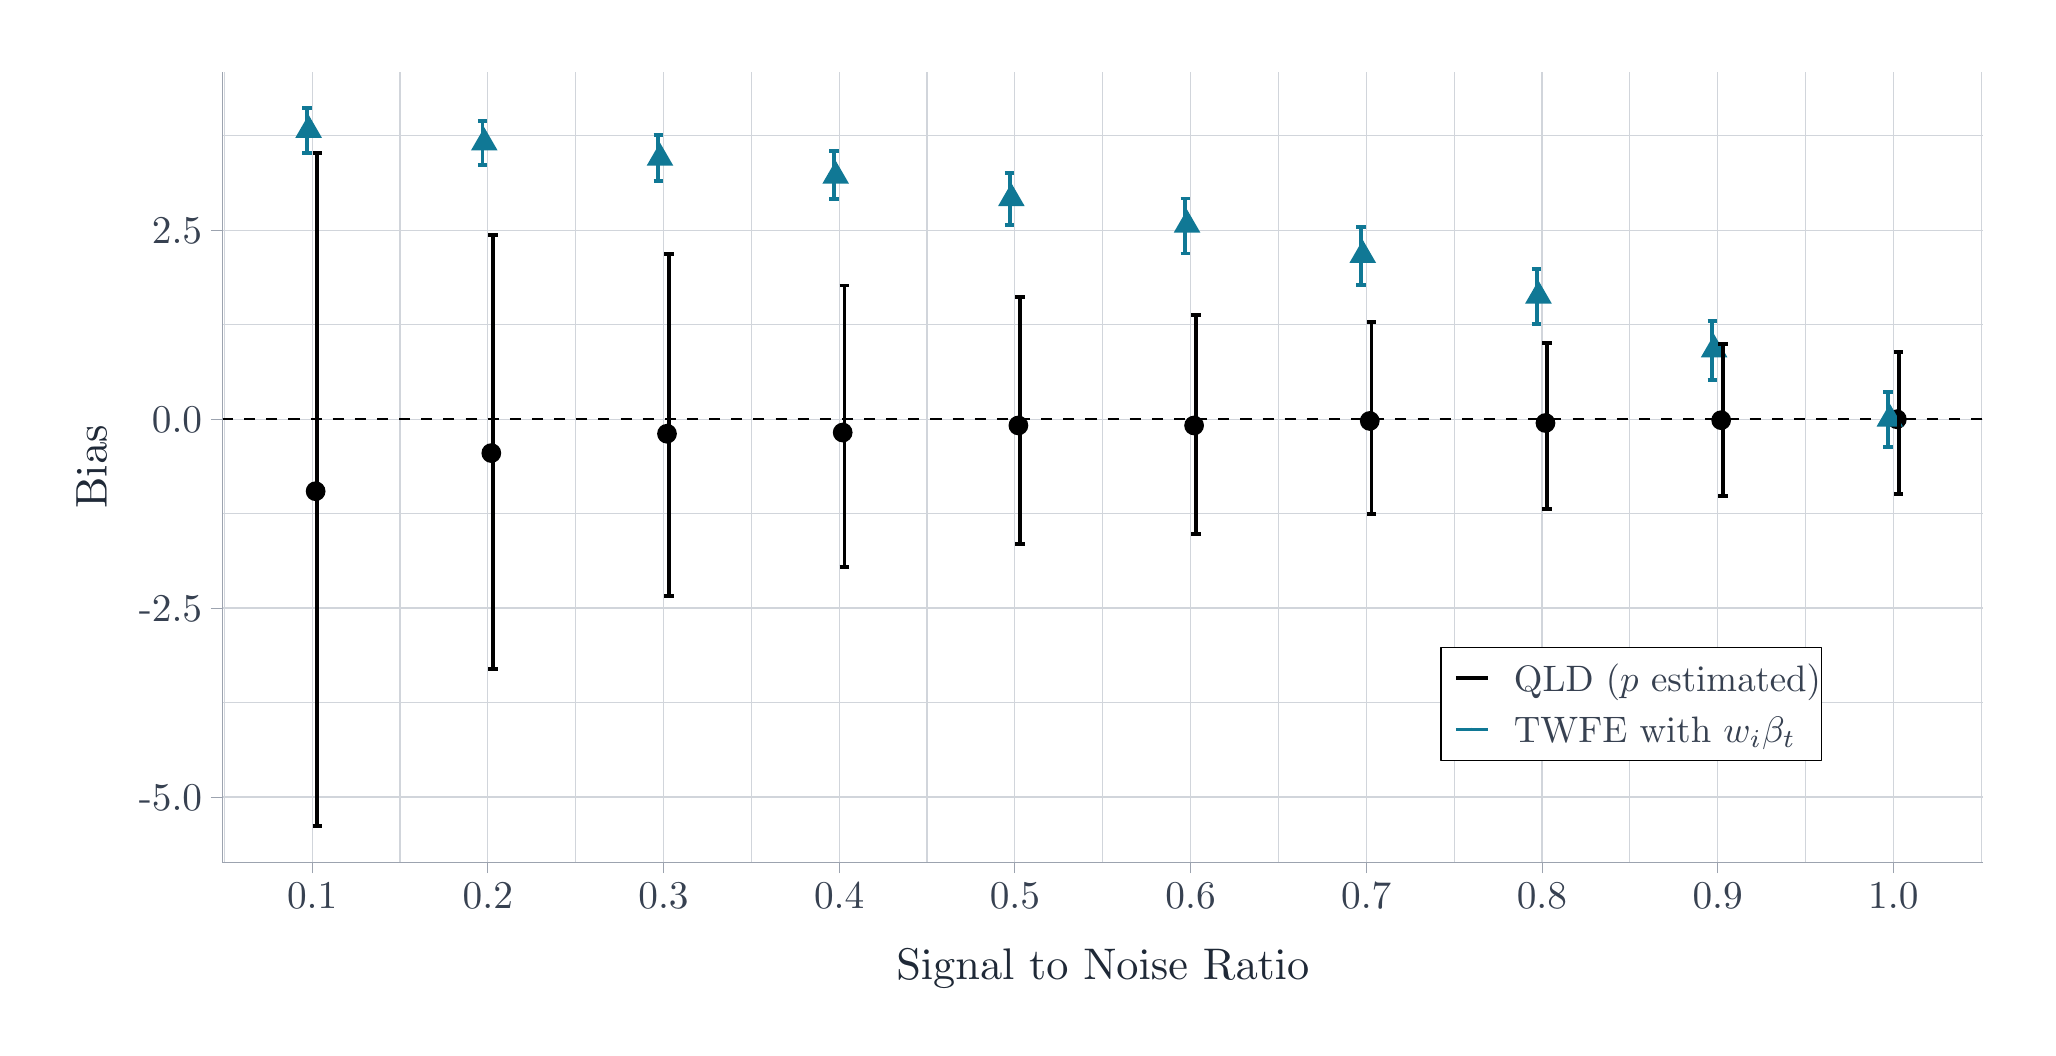
\begin{tikzpicture}[x=1pt,y=1pt]
\definecolor{fillColor}{RGB}{255,255,255}
\path[use as bounding box,fill=fillColor] (0,0) rectangle (722.70,361.35);
\begin{scope}
\path[clip] (  0.00,  0.00) rectangle (722.70,361.35);
\definecolor{drawColor}{RGB}{255,255,255}

\path[draw=drawColor,line width= 0.8pt,line join=round,line cap=round,fill=fillColor] (  0.00,  0.00) rectangle (722.70,361.35);
\end{scope}
\begin{scope}
\path[clip] ( 70.23, 59.89) rectangle (706.70,345.35);
\definecolor{drawColor}{RGB}{255,255,255}
\definecolor{fillColor}{RGB}{255,255,255}

\path[draw=drawColor,line width= 0.8pt,line join=round,line cap=round,fill=fillColor] ( 70.23, 59.89) rectangle (706.70,345.35);
\definecolor{drawColor}{RGB}{209,213,219}

\path[draw=drawColor,line width= 0.4pt,line join=round] ( 70.23,117.50) --
	(706.70,117.50);

\path[draw=drawColor,line width= 0.4pt,line join=round] ( 70.23,185.77) --
	(706.70,185.77);

\path[draw=drawColor,line width= 0.4pt,line join=round] ( 70.23,254.04) --
	(706.70,254.04);

\path[draw=drawColor,line width= 0.4pt,line join=round] ( 70.23,322.31) --
	(706.70,322.31);

\path[draw=drawColor,line width= 0.4pt,line join=round] ( 71.04, 59.89) --
	( 71.04,345.35);

\path[draw=drawColor,line width= 0.4pt,line join=round] (134.53, 59.89) --
	(134.53,345.35);

\path[draw=drawColor,line width= 0.4pt,line join=round] (198.01, 59.89) --
	(198.01,345.35);

\path[draw=drawColor,line width= 0.4pt,line join=round] (261.50, 59.89) --
	(261.50,345.35);

\path[draw=drawColor,line width= 0.4pt,line join=round] (324.98, 59.89) --
	(324.98,345.35);

\path[draw=drawColor,line width= 0.4pt,line join=round] (388.47, 59.89) --
	(388.47,345.35);

\path[draw=drawColor,line width= 0.4pt,line join=round] (451.95, 59.89) --
	(451.95,345.35);

\path[draw=drawColor,line width= 0.4pt,line join=round] (515.44, 59.89) --
	(515.44,345.35);

\path[draw=drawColor,line width= 0.4pt,line join=round] (578.92, 59.89) --
	(578.92,345.35);

\path[draw=drawColor,line width= 0.4pt,line join=round] (642.41, 59.89) --
	(642.41,345.35);

\path[draw=drawColor,line width= 0.4pt,line join=round] (705.89, 59.89) --
	(705.89,345.35);

\path[draw=drawColor,line width= 0.4pt,line join=round] ( 70.23, 83.36) --
	(706.70, 83.36);

\path[draw=drawColor,line width= 0.4pt,line join=round] ( 70.23,151.63) --
	(706.70,151.63);

\path[draw=drawColor,line width= 0.4pt,line join=round] ( 70.23,219.90) --
	(706.70,219.90);

\path[draw=drawColor,line width= 0.4pt,line join=round] ( 70.23,288.17) --
	(706.70,288.17);

\path[draw=drawColor,line width= 0.4pt,line join=round] (102.78, 59.89) --
	(102.78,345.35);

\path[draw=drawColor,line width= 0.4pt,line join=round] (166.27, 59.89) --
	(166.27,345.35);

\path[draw=drawColor,line width= 0.4pt,line join=round] (229.75, 59.89) --
	(229.75,345.35);

\path[draw=drawColor,line width= 0.4pt,line join=round] (293.24, 59.89) --
	(293.24,345.35);

\path[draw=drawColor,line width= 0.4pt,line join=round] (356.72, 59.89) --
	(356.72,345.35);

\path[draw=drawColor,line width= 0.4pt,line join=round] (420.21, 59.89) --
	(420.21,345.35);

\path[draw=drawColor,line width= 0.4pt,line join=round] (483.70, 59.89) --
	(483.70,345.35);

\path[draw=drawColor,line width= 0.4pt,line join=round] (547.18, 59.89) --
	(547.18,345.35);

\path[draw=drawColor,line width= 0.4pt,line join=round] (610.67, 59.89) --
	(610.67,345.35);

\path[draw=drawColor,line width= 0.4pt,line join=round] (674.15, 59.89) --
	(674.15,345.35);
\definecolor{drawColor}{RGB}{0,0,0}

\path[draw=drawColor,line width= 0.6pt,dash pattern=on 4pt off 4pt ,line join=round] ( 70.23,219.90) -- (706.70,219.90);
\definecolor{fillColor}{RGB}{0,0,0}

\path[fill=fillColor] (104.05,193.84) circle (  3.57);

\path[fill=fillColor] (167.54,207.63) circle (  3.57);

\path[fill=fillColor] (231.02,214.62) circle (  3.57);

\path[fill=fillColor] (294.51,215.05) circle (  3.57);

\path[fill=fillColor] (357.99,217.61) circle (  3.57);

\path[fill=fillColor] (421.48,217.60) circle (  3.57);

\path[fill=fillColor] (484.96,219.24) circle (  3.57);

\path[fill=fillColor] (548.45,218.49) circle (  3.57);

\path[fill=fillColor] (611.94,219.51) circle (  3.57);

\path[fill=fillColor] (675.42,219.86) circle (  3.57);
\definecolor{fillColor}{RGB}{16,120,149}

\path[fill=fillColor] (101.51,329.88) --
	(106.32,321.56) --
	( 96.71,321.56) --
	cycle;

\path[fill=fillColor] (165.00,325.32) --
	(169.80,316.99) --
	(160.19,316.99) --
	cycle;

\path[fill=fillColor] (228.48,319.81) --
	(233.29,311.49) --
	(223.68,311.49) --
	cycle;

\path[fill=fillColor] (291.97,313.30) --
	(296.78,304.98) --
	(287.16,304.98) --
	cycle;

\path[fill=fillColor] (355.45,305.20) --
	(360.26,296.88) --
	(350.65,296.88) --
	cycle;

\path[fill=fillColor] (418.94,295.62) --
	(423.75,287.30) --
	(414.13,287.30) --
	cycle;

\path[fill=fillColor] (482.43,284.70) --
	(487.23,276.37) --
	(477.62,276.37) --
	cycle;

\path[fill=fillColor] (545.91,269.99) --
	(550.72,261.67) --
	(541.10,261.67) --
	cycle;

\path[fill=fillColor] (609.40,250.54) --
	(614.20,242.22) --
	(604.59,242.22) --
	cycle;

\path[fill=fillColor] (672.88,225.51) --
	(677.69,217.19) --
	(668.08,217.19) --
	cycle;

\path[draw=drawColor,line width= 1.4pt,line join=round] (102.97,316.11) --
	(106.40,316.11);

\path[draw=drawColor,line width= 1.4pt,line join=round] (104.69,316.11) --
	(104.69, 72.86);

\path[draw=drawColor,line width= 1.4pt,line join=round] (102.97, 72.86) --
	(106.40, 72.86);

\path[draw=drawColor,line width= 1.4pt,line join=round] (166.46,286.32) --
	(169.89,286.32);

\path[draw=drawColor,line width= 1.4pt,line join=round] (168.17,286.32) --
	(168.17,129.71);

\path[draw=drawColor,line width= 1.4pt,line join=round] (166.46,129.71) --
	(169.89,129.71);

\path[draw=drawColor,line width= 1.4pt,line join=round] (229.94,279.64) --
	(233.37,279.64);

\path[draw=drawColor,line width= 1.4pt,line join=round] (231.66,279.64) --
	(231.66,155.85);

\path[draw=drawColor,line width= 1.4pt,line join=round] (229.94,155.85) --
	(233.37,155.85);

\path[draw=drawColor,line width= 1.4pt,line join=round] (293.43,268.16) --
	(296.86,268.16);

\path[draw=drawColor,line width= 1.4pt,line join=round] (295.14,268.16) --
	(295.14,166.38);

\path[draw=drawColor,line width= 1.4pt,line join=round] (293.43,166.38) --
	(296.86,166.38);

\path[draw=drawColor,line width= 1.4pt,line join=round] (356.91,264.15) --
	(360.34,264.15);

\path[draw=drawColor,line width= 1.4pt,line join=round] (358.63,264.15) --
	(358.63,174.90);

\path[draw=drawColor,line width= 1.4pt,line join=round] (356.91,174.90) --
	(360.34,174.90);

\path[draw=drawColor,line width= 1.4pt,line join=round] (420.40,257.47) --
	(423.83,257.47);

\path[draw=drawColor,line width= 1.4pt,line join=round] (422.11,257.47) --
	(422.11,178.42);

\path[draw=drawColor,line width= 1.4pt,line join=round] (420.40,178.42) --
	(423.83,178.42);

\path[draw=drawColor,line width= 1.4pt,line join=round] (483.89,254.90) --
	(487.31,254.90);

\path[draw=drawColor,line width= 1.4pt,line join=round] (485.60,254.90) --
	(485.60,185.73);

\path[draw=drawColor,line width= 1.4pt,line join=round] (483.89,185.73) --
	(487.31,185.73);

\path[draw=drawColor,line width= 1.4pt,line join=round] (547.37,247.28) --
	(550.80,247.28);

\path[draw=drawColor,line width= 1.4pt,line join=round] (549.08,247.28) --
	(549.08,187.44);

\path[draw=drawColor,line width= 1.4pt,line join=round] (547.37,187.44) --
	(550.80,187.44);

\path[draw=drawColor,line width= 1.4pt,line join=round] (610.86,247.12) --
	(614.28,247.12);

\path[draw=drawColor,line width= 1.4pt,line join=round] (612.57,247.12) --
	(612.57,192.02);

\path[draw=drawColor,line width= 1.4pt,line join=round] (610.86,192.02) --
	(614.28,192.02);

\path[draw=drawColor,line width= 1.4pt,line join=round] (674.34,244.08) --
	(677.77,244.08);

\path[draw=drawColor,line width= 1.4pt,line join=round] (676.06,244.08) --
	(676.06,192.90);

\path[draw=drawColor,line width= 1.4pt,line join=round] (674.34,192.90) --
	(677.77,192.90);
\definecolor{drawColor}{RGB}{16,120,149}

\path[draw=drawColor,line width= 1.4pt,line join=round] ( 99.16,332.37) --
	(102.59,332.37);

\path[draw=drawColor,line width= 1.4pt,line join=round] (100.88,332.37) --
	(100.88,316.12);

\path[draw=drawColor,line width= 1.4pt,line join=round] ( 99.16,316.12) --
	(102.59,316.12);

\path[draw=drawColor,line width= 1.4pt,line join=round] (162.65,327.76) --
	(166.08,327.76);

\path[draw=drawColor,line width= 1.4pt,line join=round] (164.36,327.76) --
	(164.36,311.57);

\path[draw=drawColor,line width= 1.4pt,line join=round] (162.65,311.57) --
	(166.08,311.57);

\path[draw=drawColor,line width= 1.4pt,line join=round] (226.14,322.46) --
	(229.56,322.46);

\path[draw=drawColor,line width= 1.4pt,line join=round] (227.85,322.46) --
	(227.85,305.96);

\path[draw=drawColor,line width= 1.4pt,line join=round] (226.14,305.96) --
	(229.56,305.96);

\path[draw=drawColor,line width= 1.4pt,line join=round] (289.62,316.74) --
	(293.05,316.74);

\path[draw=drawColor,line width= 1.4pt,line join=round] (291.33,316.74) --
	(291.33,299.38);

\path[draw=drawColor,line width= 1.4pt,line join=round] (289.62,299.38) --
	(293.05,299.38);

\path[draw=drawColor,line width= 1.4pt,line join=round] (353.11,308.77) --
	(356.53,308.77);

\path[draw=drawColor,line width= 1.4pt,line join=round] (354.82,308.77) --
	(354.82,289.96);

\path[draw=drawColor,line width= 1.4pt,line join=round] (353.11,289.96) --
	(356.53,289.96);

\path[draw=drawColor,line width= 1.4pt,line join=round] (416.59,299.63) --
	(420.02,299.63);

\path[draw=drawColor,line width= 1.4pt,line join=round] (418.31,299.63) --
	(418.31,279.76);

\path[draw=drawColor,line width= 1.4pt,line join=round] (416.59,279.76) --
	(420.02,279.76);

\path[draw=drawColor,line width= 1.4pt,line join=round] (480.08,289.29) --
	(483.50,289.29);

\path[draw=drawColor,line width= 1.4pt,line join=round] (481.79,289.29) --
	(481.79,268.39);

\path[draw=drawColor,line width= 1.4pt,line join=round] (480.08,268.39) --
	(483.50,268.39);

\path[draw=drawColor,line width= 1.4pt,line join=round] (543.56,274.23) --
	(546.99,274.23);

\path[draw=drawColor,line width= 1.4pt,line join=round] (545.28,274.23) --
	(545.28,254.30);

\path[draw=drawColor,line width= 1.4pt,line join=round] (543.56,254.30) --
	(546.99,254.30);

\path[draw=drawColor,line width= 1.4pt,line join=round] (607.05,255.23) --
	(610.48,255.23);

\path[draw=drawColor,line width= 1.4pt,line join=round] (608.76,255.23) --
	(608.76,234.11);

\path[draw=drawColor,line width= 1.4pt,line join=round] (607.05,234.11) --
	(610.48,234.11);

\path[draw=drawColor,line width= 1.4pt,line join=round] (670.53,229.56) --
	(673.96,229.56);

\path[draw=drawColor,line width= 1.4pt,line join=round] (672.25,229.56) --
	(672.25,209.81);

\path[draw=drawColor,line width= 1.4pt,line join=round] (670.53,209.81) --
	(673.96,209.81);
\end{scope}
\begin{scope}
\path[clip] (  0.00,  0.00) rectangle (722.70,361.35);
\definecolor{drawColor}{RGB}{156,163,175}

\path[draw=drawColor,line width= 0.3pt,line join=round] ( 70.23, 59.89) --
	( 70.23,345.35);
\end{scope}
\begin{scope}
\path[clip] (  0.00,  0.00) rectangle (722.70,361.35);
\definecolor{drawColor}{RGB}{55,65,81}

\node[text=drawColor,anchor=base east,inner sep=0pt, outer sep=0pt, scale=  1.42] at ( 63.03, 78.46) {-5.0};

\node[text=drawColor,anchor=base east,inner sep=0pt, outer sep=0pt, scale=  1.42] at ( 63.03,146.73) {-2.5};

\node[text=drawColor,anchor=base east,inner sep=0pt, outer sep=0pt, scale=  1.42] at ( 63.03,215.00) {0.0};

\node[text=drawColor,anchor=base east,inner sep=0pt, outer sep=0pt, scale=  1.42] at ( 63.03,283.28) {2.5};
\end{scope}
\begin{scope}
\path[clip] (  0.00,  0.00) rectangle (722.70,361.35);
\definecolor{drawColor}{RGB}{156,163,175}

\path[draw=drawColor,line width= 0.3pt,line join=round] ( 66.23, 83.36) --
	( 70.23, 83.36);

\path[draw=drawColor,line width= 0.3pt,line join=round] ( 66.23,151.63) --
	( 70.23,151.63);

\path[draw=drawColor,line width= 0.3pt,line join=round] ( 66.23,219.90) --
	( 70.23,219.90);

\path[draw=drawColor,line width= 0.3pt,line join=round] ( 66.23,288.17) --
	( 70.23,288.17);
\end{scope}
\begin{scope}
\path[clip] (  0.00,  0.00) rectangle (722.70,361.35);
\definecolor{drawColor}{RGB}{156,163,175}

\path[draw=drawColor,line width= 0.3pt,line join=round] ( 70.23, 59.89) --
	(706.70, 59.89);
\end{scope}
\begin{scope}
\path[clip] (  0.00,  0.00) rectangle (722.70,361.35);
\definecolor{drawColor}{RGB}{156,163,175}

\path[draw=drawColor,line width= 0.3pt,line join=round] (102.78, 55.89) --
	(102.78, 59.89);

\path[draw=drawColor,line width= 0.3pt,line join=round] (166.27, 55.89) --
	(166.27, 59.89);

\path[draw=drawColor,line width= 0.3pt,line join=round] (229.75, 55.89) --
	(229.75, 59.89);

\path[draw=drawColor,line width= 0.3pt,line join=round] (293.24, 55.89) --
	(293.24, 59.89);

\path[draw=drawColor,line width= 0.3pt,line join=round] (356.72, 55.89) --
	(356.72, 59.89);

\path[draw=drawColor,line width= 0.3pt,line join=round] (420.21, 55.89) --
	(420.21, 59.89);

\path[draw=drawColor,line width= 0.3pt,line join=round] (483.70, 55.89) --
	(483.70, 59.89);

\path[draw=drawColor,line width= 0.3pt,line join=round] (547.18, 55.89) --
	(547.18, 59.89);

\path[draw=drawColor,line width= 0.3pt,line join=round] (610.67, 55.89) --
	(610.67, 59.89);

\path[draw=drawColor,line width= 0.3pt,line join=round] (674.15, 55.89) --
	(674.15, 59.89);
\end{scope}
\begin{scope}
\path[clip] (  0.00,  0.00) rectangle (722.70,361.35);
\definecolor{drawColor}{RGB}{55,65,81}

\node[text=drawColor,anchor=base,inner sep=0pt, outer sep=0pt, scale=  1.42] at (102.78, 42.89) {0.1};

\node[text=drawColor,anchor=base,inner sep=0pt, outer sep=0pt, scale=  1.42] at (166.27, 42.89) {0.2};

\node[text=drawColor,anchor=base,inner sep=0pt, outer sep=0pt, scale=  1.42] at (229.75, 42.89) {0.3};

\node[text=drawColor,anchor=base,inner sep=0pt, outer sep=0pt, scale=  1.42] at (293.24, 42.89) {0.4};

\node[text=drawColor,anchor=base,inner sep=0pt, outer sep=0pt, scale=  1.42] at (356.72, 42.89) {0.5};

\node[text=drawColor,anchor=base,inner sep=0pt, outer sep=0pt, scale=  1.42] at (420.21, 42.89) {0.6};

\node[text=drawColor,anchor=base,inner sep=0pt, outer sep=0pt, scale=  1.42] at (483.70, 42.89) {0.7};

\node[text=drawColor,anchor=base,inner sep=0pt, outer sep=0pt, scale=  1.42] at (547.18, 42.89) {0.8};

\node[text=drawColor,anchor=base,inner sep=0pt, outer sep=0pt, scale=  1.42] at (610.67, 42.89) {0.9};

\node[text=drawColor,anchor=base,inner sep=0pt, outer sep=0pt, scale=  1.42] at (674.15, 42.89) {1.0};
\end{scope}
\begin{scope}
\path[clip] (  0.00,  0.00) rectangle (722.70,361.35);
\definecolor{drawColor}{RGB}{31,41,55}

\node[text=drawColor,anchor=base,inner sep=0pt, outer sep=0pt, scale=  1.60] at (388.47, 17.56) {Signal to Noise Ratio};
\end{scope}
\begin{scope}
\path[clip] (  0.00,  0.00) rectangle (722.70,361.35);
\definecolor{drawColor}{RGB}{31,41,55}

\node[text=drawColor,rotate= 90.00,anchor=base,inner sep=0pt, outer sep=0pt, scale=  1.60] at ( 28.57,202.62) {Bias};
\end{scope}
\begin{scope}
\path[clip] (  0.00,  0.00) rectangle (722.70,361.35);
\definecolor{drawColor}{RGB}{0,0,0}
\definecolor{fillColor}{RGB}{255,255,255}

\path[draw=drawColor,line width= 0.6pt,line join=round,line cap=round,fill=fillColor] (510.59, 96.53) rectangle (648.22,137.43);
\end{scope}
\begin{scope}
\path[clip] (  0.00,  0.00) rectangle (722.70,361.35);
\definecolor{drawColor}{RGB}{255,255,255}
\definecolor{fillColor}{RGB}{255,255,255}

\path[draw=drawColor,line width= 0.8pt,line join=round,line cap=round,fill=fillColor] (514.59,118.98) rectangle (529.05,133.43);
\end{scope}
\begin{scope}
\path[clip] (  0.00,  0.00) rectangle (722.70,361.35);
\definecolor{fillColor}{RGB}{0,0,0}

\path[fill=fillColor] (521.82,126.21) circle (  0.36);
\end{scope}
\begin{scope}
\path[clip] (  0.00,  0.00) rectangle (722.70,361.35);
\definecolor{drawColor}{RGB}{0,0,0}

\path[draw=drawColor,line width= 1.4pt,line join=round] (516.04,126.21) -- (527.60,126.21);
\end{scope}
\begin{scope}
\path[clip] (  0.00,  0.00) rectangle (722.70,361.35);
\definecolor{drawColor}{RGB}{255,255,255}
\definecolor{fillColor}{RGB}{255,255,255}

\path[draw=drawColor,line width= 0.8pt,line join=round,line cap=round,fill=fillColor] (514.59,100.53) rectangle (529.05,114.98);
\end{scope}
\begin{scope}
\path[clip] (  0.00,  0.00) rectangle (722.70,361.35);
\definecolor{fillColor}{RGB}{16,120,149}

\path[fill=fillColor] (521.82,108.31) --
	(522.30,107.48) --
	(521.34,107.48) --
	cycle;
\end{scope}
\begin{scope}
\path[clip] (  0.00,  0.00) rectangle (722.70,361.35);
\definecolor{drawColor}{RGB}{16,120,149}

\path[draw=drawColor,line width= 1.4pt,line join=round] (516.04,107.75) -- (527.60,107.75);
\end{scope}
\begin{scope}
\path[clip] (  0.00,  0.00) rectangle (722.70,361.35);
\definecolor{drawColor}{RGB}{55,65,81}

\node[text=drawColor,anchor=base west,inner sep=0pt, outer sep=0pt, scale=  1.33] at (537.05,121.62) {QLD ($p$ estimated)};
\end{scope}
\begin{scope}
\path[clip] (  0.00,  0.00) rectangle (722.70,361.35);
\definecolor{drawColor}{RGB}{55,65,81}

\node[text=drawColor,anchor=base west,inner sep=0pt, outer sep=0pt, scale=  1.33] at (537.05,103.16) {TWFE with $\bm{w}_i \beta_t$};
\end{scope}
\end{tikzpicture}
